\documentclass[17pt]{beamer}
%\documentclass[handout]{beamer} %Makes Handouts
\usetheme{Singapore} %Gray with fade at top
\useoutertheme[subsection=false]{miniframes} %Supppress subsection in header
\useinnertheme{rectangles} %Itemize/Enumerate boxes
\usecolortheme{seagull} %Color theme
\usecolortheme{rose} %Inner color theme

\definecolor{light-gray}{gray}{0.75}
\definecolor{dark-gray}{gray}{0.55}
\setbeamercolor{item}{fg=light-gray}
\setbeamercolor{enumerate item}{fg=dark-gray}

\setbeamertemplate{navigation symbols}{}
\setbeamertemplate{mini frames}{}
%\setbeamercovered{dynamics}
\setbeamerfont*{title}{size=\Large,series=\bfseries}
\setbeamerfont{footnote}{size=\tiny}

%\setbeameroption{notes on second screen} %Dual-Screen Notes
%\setbeameroption{show only notes} %Notes Output

\setbeamertemplate{frametitle}{\vspace{.5em}\bfseries\insertframetitle}
\newcommand{\heading}[1]{\noindent \textbf{#1}\\ \vspace{1em}}
\newcommand{\questions}{\frame{{\large Questions?}}}

\usepackage{bbding,color,multirow,times,ccaption,tabularx,graphicx,verbatim,booktabs}
\usepackage{colortbl} %Table overlays
\usepackage[english]{babel}
\usepackage[latin1]{inputenc}
\usepackage[T1]{fontenc}
\usepackage{lmodern}
\usepackage{alltt}

\usepackage{tikz}
\usetikzlibrary{shapes,arrows,decorations.pathreplacing,calc}


\author[]{Thomas J. Leeper}
\institute{
  Government Department\\London School of Economics and Political Science
}


\title{Session II\\Examples and Paradigms}

\date[]{}

\begin{document}

\frame{\titlepage}

\frame{\tableofcontents}


\frame{

\frametitle{Analysis}

See website for
\begin{itemize}
\item Data from yesterday's activity
\item R code for basic experimental analysis
\item Stata code for basic experimental analysis
\end{itemize}
}


\frame{

\frametitle{{\normalsize Aside: Complex Designs}}

\small

\begin{itemize}
\item An experiment can have any number of conditions
	\begin{itemize}\footnotesize
	\item Up to the limits of sample size
	\item More than 8--10 conditions is typically unwieldy
	\end{itemize}
\item Still analyze complex designs using regression, but focus on pairwise comparisons to estimates SATEs
	\begin{itemize}\footnotesize
	\item Treatment--treatment, or treatment-control
	\item Without control group, we don't know which treatment(s) affected the outcome
	\end{itemize}
\end{itemize}

}




\section[Theory]{From Theory to Design}
\frame{\tableofcontents[currentsection]}
% deriving hypotheses from theory and manipulations from hypotheses


\frame{

\frametitle{{\large What makes a good research question?}}

\small

KKV's two criteria:

\begin{enumerate}
\item Politically important
\item Contribute to scientific literature
\vspace{0.25em}
\item<2-> Personally interesting
\item<2-> Unresolved
\item<3-> For experiments, \textit{forward} in nature
\end{enumerate}
}


\frame{

\frametitle{{\normalsize Experiments are good at answering ``what if'' questions}}

\normalsize

\begin{itemize}\itemsep0.5em
\item Forward causal questions
	\begin{itemize}
	\item Can X cause Y?
	\item What effects does X have?
	\end{itemize}
\item<2-> Backward causal questions
	\begin{itemize}
	\item What causes Y?
	\item How much of Y is attributable to X?
	\end{itemize}
\item<3-> Even though answering ``forward'' causal question, we start with an outcome concept
\end{itemize}
}




\frame{

\frametitle{Hypothesis Testing}

\begin{itemize}\itemsep0.5em
\item From theory, we derive testable hypotheses
\begin{itemize}
\item Hypotheses are expectations about differences in outcomes across levels of a putatively causal variable
\item Hypothesis must be testable by an SATE
\end{itemize}
\item Manipulations are developed to create variation in that causal variable
\end{itemize}

}


\frame{

\frametitle{{\normalsize Example: News Framing}}

\small

\begin{itemize}
\item Theory: Presentation of news affects opinion
\item Hypotheses:
	\begin{itemize}\footnotesize
	\item News emphasizing free speech increases support for a hate group rally
	\item News emphasizing public safety decreases support for a hate group rally
	\end{itemize}
\item Manipulation:
	\begin{itemize}\footnotesize
	\item Control group: no information
	\item Free speech group: article emphasizing rights
	\item Public safety group: article emphasizing safety
	\end{itemize}
\end{itemize}

}




\frame{

\frametitle{{\normalsize Example: Partisan Identity}}

\small

\begin{itemize}
\item Theory: Strength of partisan identity affects tendency to accept party position
\item Hypotheses:
	\begin{itemize}\small
	\item Strong partisans are more likely to accept their party's position on an issue
	\end{itemize}
\item Manipulation:
	\begin{itemize}\small
	\item Control group: no manipulation
	\item ``Univalent'' condition
	\item ``Ambivalent'' condition
	\end{itemize}
\end{itemize}

}


\frame[label=ambivalentpartisan]{

\frametitle{\textbf{\only<1>{Univalent}\only<2>{Ambivalent}}}

\footnotesize

These days, Democrats and Republicans differ from one another considerably. The two groups seem to be growing further and further apart, not only in terms of their opinions but also their lifestyles. Earlier in the survey, you said you tend to identify as a \textit{Democrat/ Republican}. Please take a few minutes to think about what you like about \textit{Democrats/ Republicans} compared to the \textit{Republicans/ Democrats}. Think of 2 to 3 things you especially like best about \textbf{\only<1>{your party}\only<2>{the other party}}. Then think of 2 to 3 things you especially dislike about \textbf{\only<2>{your party}\only<1>{the other party}}. Now please write those thoughts in the space below.

}



\frame{

\frametitle{Hypothesis Testing}

\begin{itemize}
\item Derive experimental design from hypotheses
\item Experimental ``factors'' are expressions of hypotheses as randomized groups
\item What intervention each group receives depends on hypotheses
	\begin{itemize}
	\item presence/absence
	\item levels/doses
	\item qualitative variations
	\end{itemize}
\end{itemize}

}


\frame{

\frametitle{{\normalsize Ex.: Presence/Absence}}

\small

\begin{itemize}
\item Theory: Negative campaigning reduces support for the party described negatively.
\item Hypothesis: Exposure to a negative advertisement criticizing a party reduces support for that party.
\item Manipulation:
	\begin{itemize}\small 
	\item Control group receives no advertisement. 
	\item Treatment group watches a video containing a negative ad describing a party.
	\end{itemize}
\end{itemize}

}


\frame{

\frametitle{{\normalsize Ex.: Levels/doses}}

\small

\begin{itemize}\itemsep-0.2em
\item Theory: Negative campaigning reduces support for the party described negatively.
\item Hypothesis: Exposure to higher levels of negative advertising criticizing a party reduces support for that party.
\item Manipulation:
	\begin{itemize}\footnotesize
	\item Control group receives no advertisement. 
	\item Treatment group 1 watches a video containing 1 negative ad describing a party.
	\item Treatment group 2 watches a video containing 2 negative ads describing a party.
	\item Treatment group 3 watches a video containing 3 negative ads describing a party.
	\item etc.
	\end{itemize}
\end{itemize}

}


\frame{

\frametitle{{\normalsize Ex.: Qualitative variation}}

\small

\begin{itemize}
\item Theory: Negative campaigning reduces support for the party described negatively.
\item Hypothesis: Exposure to a negative advertisement criticizing a party reduces support for that party, while a positive advertisement has no effect.
\item Manipulation:
	\begin{itemize}\footnotesize
	\item Control group receives no advertisement. 
	\item Negative treatment group watches a video containing a negative ad describing a party.
	\item Positive treatment group watches a video containing a positive ad describing a party.
	\end{itemize}
\end{itemize}

}

\questions

\frame{

\frametitle{Share your TESS Examples}

In groups of 4--5, share your TESS examples
\begin{itemize}
\item What was the researcher's question?
\item How did they test it experimentally?
\item What was interesting or surprising about the designs?
\end{itemize}

Take about 7--8 minutes.

}





% Talk about protocol and preregistration

\frame{

\frametitle{Protocol}

Protocol is the complete planning document for how to design, implement, and analyze an experiment.\footnote{Thomas J. Leeper. 2011. ``The Use of Protocol in the Design and Reporting of Experiments.'' \textit{The Experimental Political Scientist}.}

}

\frame{

\frametitle{{\normalsize Protocol}}


\small

\begin{enumerate}\itemsep-0.2em
\item Theory/hypotheses
\item Instrumentation
	\begin{itemize}
	\item Manipulation(s)
	\item Outcome(s)
	\item Covariate(s)
	\item Manipulation check(s)
	\end{itemize}
\item Sampling
\item Implementation
\item Analysis
\end{enumerate}
}

\frame{

\frametitle{Why bother?}

\begin{itemize}\itemsep0.5em
\item<2-> Be clear to yourself what you're trying to do before you do it
\item<3-> Assess the literature for best practices
\item<4-> Highlight areas in need of pilot testing
\item<5-> Economize questionnaire development
\item<6-> Study preregistration
\end{itemize}

}


\frame{

\frametitle{Activity!}

\begin{itemize}\itemsep0.5em
\item How do we know if an experiment is any good?
\item Talk with a partner for about 3 minutes
\item Try to develop some criteria that allow you to evaluate ``what makes for a good experiment?'' 
\end{itemize}

}


\frame{

\frametitle{Some possible criteria}

\small

\begin{itemize}\itemsep-0.2em
\item Significant results
\item Face validity
\item Coherent for respondents
\item Non-obvious to respondents
\item Simple
\item Indirect/unobtrusive
\item Validated by prior work
\item Innovative/creative
\item \dots
\end{itemize}

}


\questions

\section{Assessing Treatments}
\frame{\tableofcontents[currentsection]}


\frame{

\begin{quote}\large
The best criterion for evaluating the quality of an experiment is whether it manipulated the intended independent variable and controlled everything else by design.
\end{quote}
\onslide<2->{\small\hspace{5em} --Thomas J. Leeper (5 July 2016)}

}

\frame{

\frametitle{How do we know we manipulated what we think we manipulated?}

\small

\begin{itemize}
\item<2-> Outcomes are affected consistent with theory
\item<3-> Before the study using \textit{pilot testing} (or \emph{pretesting})
\item<4-> During the study, using \emph{manipulation checks}
\item<5-> During the study, using \emph{placebos}
\item<6-> During the study, using \textit{non-equivalent outcomes}
\end{itemize}
}

\frame{

\frametitle{I. Outcomes Affected}

\begin{itemize}\itemsep0.5em
\item Follows a circular logic!
\item Doesn't tell us anything if we hypothesize null effects
\end{itemize}

}


\frame{

\frametitle{II. Pilot Testing}

\small

\begin{itemize}\itemsep0.2em
\item Goal: establish construct validity of manipulation
\item Assess whether a set of possible manipulations affect a measure of the \textit{independent} variable
\item<2-> Example:
	\begin{itemize}
	\item Goal: Manipulate the ``strength'' of an argument
	\item Write several arguments
	\item Ask pilot test respondents to report how strong each one was
	\end{itemize}
\end{itemize}

}

\frame{

\frametitle{III. Manipulation Checks}

\small

\begin{itemize}\itemsep0.2em
\item Manipulation checks are items added post-treatment, post-outcome that assess whether the \textit{independent} variable was affected by treatment
\item We typically talk about manipulations as directly setting the value of $X$, but in practice we are typically manipulating something \textit{that we think} strongly modifies $X$
\item<2-> Example: information manipulations aim to modify knowledge or beliefs, but are necessarily imperfect at doing so
\end{itemize}

}

\frame{

\frametitle{\normalsize Manipulation check example\footnote{Leeper \& Slothuus. n.d. ``Can Citizens Be Framed?'' Available from: \url{http://thomasleeper.com/research.html}.}}

\begin{enumerate}
\item Treatment 1: Supply Information
\item Manipulation check 1: measure beliefs
\item Treatment 2: Prime a set of considerations
\item Outcome: Measure opinion
\item Manipulation check 2: measure dimension salience
\end{enumerate}

}


\frame{

\frametitle{{\normalsize Some Best Practices}}


\begin{itemize}\itemsep0.5em
\item<2-> Manipulation checks should be innocuous
	\begin{itemize}
	\item Shouldn't modify independent variable
	\item Shouldn't modify outcome variable
	\end{itemize}
\item<3-> Generally, measure post-outcome
\item<4-> Measure both what you wanted to manipulate \textit{and} what you didn't want to manipulate
	\begin{itemize}
	\item Most treatments are \textit{compound}!
	\end{itemize}
\end{itemize}

}

\frame{

\frametitle{IV. Placebos}

\begin{itemize}\itemsep0.5em
\item Include an experimental condition that \textit{does not} manipulate the variable of interest (but might affect the outcome)
\item<2-> Example:
	\begin{itemize}
	\item Study whether risk-related arguments about climate change increase support for a climate change policy
	\item Placebo condition: control article with risk-related arguments about non-environmental issue (e.g., terrorism)
	\end{itemize}
\end{itemize}

}

\frame{

\frametitle{V. Non-equivalent outcomes}

\small

\begin{itemize}\itemsep0.5em
\item Measures an outcome that \textit{should not} be affected by independent variable
\item<2-> Example:
	\begin{itemize}
	\item Assess effect of some treatment on attitudes toward group A
	\item Focal outcome: attitudes toward group A
	\item Non-equivalent outcome: attitudes toward group B
	\end{itemize}
\end{itemize}

}


\frame{

\frametitle{{\normalsize Aside: Demand Characteristics}}

\small

\begin{itemize}\itemsep0.5em
\item ``Demand characteristics'' are features of experiments that (unintentionally) imply the purpose of the study and thereby change respondents' behavior (to be consistent with theory)
\item<2-> Implications:
	\begin{itemize}\footnotesize
	\item Design experimental treatments that are non-obvious
	\item Do not disclose the purpose of the study up front\footnote{But, consider the ethics of not doing so (more Friday)}
	\end{itemize}
\end{itemize}

}





\section[Paradigms]{Common Paradigms and Examples}
\frame{\tableofcontents[currentsection]}


\frame{

\frametitle{Question Wording Designs}

\begin{itemize}
\item Kahneman and Tversky is a ``question wording'' experiment
\item Hypothesized difference in outcomes according to the decision being faced
	\begin{itemize}
	\item Risky or not risky
	\item Gains or losses
	\end{itemize}
\item Manipulation operationalizes this by asking two different questions
\item Outcome is the answer to the question
\end{itemize}

}

\frame{

\frametitle{Activity!}

\begin{itemize}
\item With a partner, identify each of the protocol elements of the experiment described by Kahneman and Tversky
\begin{enumerate}
\item Theory/hypotheses
\item Instrumentation
\item Sampling
\item Implementation
\item Analysis
\end{enumerate}
\item Report back in about 4 minutes
\end{itemize}

}



\frame{

\frametitle{``Framing'' or ``Priming'' Experiments}

Example: Schuldt et al. ```Global Warming' or `Climate Change'? Whether the Planet is Warming Depends on Question Wording.''

\vspace{1em}

What's this study about?
}


\frame{

\small

You may have heard about the idea that the world's temperature may have been \textbf{\only<1>{going up}\only<2>{changing}} over the past 100 years, a phenomenon sometimes called \textbf{\only<1>{global warming}\only<2>{climate change}}. What is your personal opinion regarding whether or not this has been happening?
	\begin{itemize}\itemsep-0.25em\footnotesize
	\item Definitely has not been happening
	\item Probably has not been happening
	\item Unsure, but leaning toward it has not been happening
	\item Not sure either way
	\item Unsure, but leaning toward it has been happening
	\item Probably has been happening
	\item Definitely has been happening
	\end{itemize}
}


\frame{

\frametitle{{\normalsize Another framing example\footnote{Singer \& Couper. 2014. ``The Effect of Question Wording on Attitudes toward Prenatal Testing and Abortion.'' \textit{Public Opinion Quarterly} 78(3): 751--760.}}}

\footnotesize

Today, tests are being developed that make it possible to detect serious genetic defects \textbf{\only<1>{before a baby is born}\only<2>{in the fetus during pregnancy}}. But so far, it is impossible either to treat or to correct most of them. If (you/your partner) were pregnant, would you want (her) to have a test to find out if the \textbf{\only<1>{baby}\only<2>{fetus}} has any serious genetic defects? (Yes/No)\\

\vspace{0.5em}

Suppose a test shows the \textbf{\only<1>{baby}\only<2>{fetus}} has a serious genetic defect. Would you, yourself, want (your partner) to have an abortion if a test shows the \textbf{\only<1>{baby}\only<2>{fetus}} has a serious genetic defect? (Yes/No)

}


\frame{

\frametitle{{\normalsize Another framing example\footnote{Bobo \& Johnson. 2004. ``A Taste for Punishment: Black and White Americans' Views on the Death Penalty and the War on Drugs.'' Du Bois Review 1(1): 151--180.}}}

\only<2>{Blacks are about 12\% of the U.S. population, but they were half of the homicide offenders last year. }Do you favor or oppose the death penalty for persons convicted of murder?

}

\frame{

\frametitle{{\normalsize Another framing example\footnote{Haider-Markel \& Joslyn. 2001. ``Gun Policy, Opinion, Tragedy, and Blame Attribution: The Conditional Influence of Issue Frames.'' \textit{Journal of Politics} 63(2): 520--543.}}}

\only<1>{Concealed handgun laws have recently received national attention. Some people have argued that law-abiding citizens have the right to protect themselves.}\only<2>{Concealed handgun laws have recently received national attention. Some people have argued that laws allowing citizens to carry concealed handguns threaten public safety because they would allow almost anyone to carry a gun almost anywhere, even onto school grounds.} What do you think about concealed handgun laws?

}


\frame{

\frametitle{Question testing}

Use question wording designs to select which survey measures we want to use

\begin{itemize}
\item Select possible question wordings
\item Select some criterion(-ia) for assessing which is better
\item Pilot test and then use the item that performs better
\end{itemize}

}


\frame{

\frametitle{{\normalsize Aside: Experimentation vs. Other Pretesting Methods}}

\small

\begin{itemize}\itemsep0.25em
\item<2-> Experiments are complementary to other pretesting methods
\item<3-> Specific value added of an experiment: optimize questions or other survey features against a specific criterion, e.g.:
	\begin{itemize}\footnotesize
	\item (Non-)Response or drop-off rates
	\item ``Don't know'' rates
	\item Item characteristics
	\item Reading times or response latencies
	\end{itemize}
\item<4-> But! Power considerations\dots
\end{itemize}

}

\frame{

\frametitle{{\normalsize Classic question testing experiment\footnote{Bishop, G.F., Tuchfarber, A. \& Oldendick, R.W. 1986. ``Opinions on Fictitious Issues: The Pressure to Answer Survey Questions.'' \textit{Public Opinion Quarterly} 50(2): 240--250.}}}

Some people feel that The 1975 Public Affairs Act should be repealed-do you agree or disagree with this idea\only<1>{?}\only<2>{, or haven't you thought much about this issue?}

}


\frame{

\frametitle{{\normalsize An example\footnote{Holbrook \& Krosnick. 2013. ``A New Question Sequence to Measure Voter Turnout in Telephone Surveys: Results of an Experiment in the 2006 {ANES} Pilot Study.'' \textit{Public Opinion Quarterly} 77: 106--123.}}}

\small

In talking to people about elections, we often find that a lot of people were not able to vote because they weren't registered, they were sick, or they just didn't have time. \only<1>{How about you--did you vote in the elections this November?}\only<2>{Which of the following statements best describes you?
    \begin{itemize}\footnotesize
    \item One, I did not vote in the November 3 election
    \item two, I thought about voting this time but didn't
    \item three, I usually vote but didn't this time
    \item four, I am sure I voted
    \end{itemize}}

}

\frame{

\frametitle{{\normalsize An Instructional Manipulation\footnote{Sturgis, Allum \& Smith. 2008. ``An Experiment on the Measurement of Political Knowledge in Surveys.'' \textit{Public Opinion Quarterly} 72(1): 90--102.}}}

\small

For the next few questions, I am going to read out some statements, and for each one, please tell me if it is true or false. If you don't know, \only<1>{just say so and we will skip to the next one}\only<2>{please just give me your best guess}.

\begin{enumerate}\footnotesize
\item Britain's electoral system is based on proportional representation.
\item MPs from different parties are on parliamentary committees.
\item The Conservatives are opposed to the ratification of a constitution for the European Union.
\end{enumerate}

}


\frame{

\frametitle{{\normalsize An Instructional Manipulation + \footnote{Prior \& Lupia. 2008. ``Money, Time, and Political Knowledge: Distinguishing Quick Recall and Political Learning Skills.'' \textit{American journal of Political Science} 52(1): 169--183.}}}

\small

\only<1>{In the next part of this study, you will be asked 14 questions about politics, public policy, and economics. Many people don't know the answers to these questions, but it is helpful for us if you answer, even if you're not sure what the correct answer is. We encourage you to take a guess on every question. At the end of this study, you will see a summary of how many questions you answered correctly.}\only<2>{We will pay you for answering questions correctly.
You will earn \$1 for every correct answer you give. So, if you answer 3 of the 14 questions correctly, you will earn \$3. If you answer 7 of the 14 questions correctly, you will earn \$7. The more questions you answer correctly, the more you will earn.}

}



\frame{

\frametitle{{\normalsize Question Order Designs}}

\small

\begin{itemize}
\item Manipulation of pre-outcome questionnaire
\item<2-> Example:
	\begin{itemize}
	\item Goal: assess influence of value salience on support for a policy
	\item Manipulate by asking different questions:
		\begin{itemize}
		\item Battery of 5 ``rights'' questions, or
		\item Battery of 5 ``life'' questions
		\end{itemize}
	\item Measure support for legalized abortion
	\end{itemize}
\item<3-> If answers to manipulated questions matter, can measure rest post-outcome
\end{itemize}

}

\frame{
	\frametitle{{\normalsize Ex. Question-as-treatment\footnote{Transue. 2007. ``Identity Salience, Identity Acceptance, and Racial Policy Attitudes: {American} National Identity as a Uniting Force.'' \textit{American Journal of Political Science} 51(1): 78--91.}}}
	

\begin{itemize}
\item \only<1,3>{How close do you feel to your ethnic or racial group?}\only<2,4>{How close do you feel to other Americans?}
\item \only<1-2>{Some people have said that taxes need to be raised to take care of pressing national needs. How willing would you be to have your taxes raised to improve education in public schools?}\only<3-4>{Some people have said that taxes need to be raised to take care of pressing national needs. How willing would you be to have your taxes raised to improve educational opportunities for minorities?}
\end{itemize}
	
}


\frame{

\frametitle{{\normalsize Ex.: Knowledge and Political Interest}}

\footnotesize

\begin{enumerate}
\item Do you happen to remember anything special that your U.S. Representative has done for your district or for the people in your district while he has been in Congress?
\item Is there any legislative bill that has come up in the House of Representatives, on which you remember how your congressman has voted in the last couple of years?
\item Now, some people seem to follow what's going on in government and public affairs most of the time, whether there's an election going on or not. Others aren't that interested. Would you say that you follow what's going on in government and public affairs most of the time, some of the time, only now and then, or hardly at all?
\end{enumerate}

}

\frame{

\frametitle{{\normalsize Ex.: Knowledge and Political Interest}}

\footnotesize

\begin{enumerate}
\item Now, some people seem to follow what's going on in government and public affairs most of the time, whether there's an election going on or not. Others aren't that interested. Would you say that you follow what's going on in government and public affairs most of the time, some of the time, only now and then, or hardly at all?
\item Do you happen to remember anything special that your U.S. Representative has done for your district or for the people in your district while he has been in Congress?
\item Is there any legislative bill that has come up in the House of Representatives, on which you remember how your congressman has voted in the last couple of years?
\end{enumerate}

}



\frame{

\frametitle{Vignettes}

\begin{itemize}
\item A ``vignette'' is a short paragraph of text describing a situation
\item Vignettes are probably the most common survey experimental paradigm, after question wording designs
\item Take many forms and increasingly encompass non-textual stimuli
\item Basically limited to web-based mode
\end{itemize}

}

\frame{

\frametitle{A classic vignette\footnote{Gilens, M. 1996. ```Race coding' and white opposition to welfare. \textit{American Political Science Review} 90(3): 593--604.}}

Now think about a \textbf{(black/white)} woman in her early thirties. She is a high school \textbf{(graduate/drop out)} with a ten-year-old child, and she has been on welfare for the past year.

\begin{itemize}\tiny
\item How likely is it that she will have more children in order to get a bigger welfare check? (1 = Very likely, \dots, 7 = Not at all likely)
\item How likely do you think it is that she will really try hard to find a job in the next year? (1 = Very likely, \dots, 7 = Not at all likely)
\end{itemize}
}


\frame{

\frametitle{Article-type vignettes}

% articles

% Nelson et al.

}


\frame{

\frametitle{Video manipulations}

% videos

}


% vignette
% text
% video


\frame{

\frametitle{{\large Some vignette considerations}}

\begin{itemize}\small
\item<2-> Comparability across conditions
	\begin{itemize}
	\item Length
	\item Readability
	\end{itemize}
\item<3-> Language proficiency
\item<4-> Length
	\begin{itemize}\small
	\item Timers
	\item Forced exposure
	\item Mouse trackers
	\end{itemize}
\item<5-> Devices
	\begin{itemize}\small
	\item Browser-specificity
	\item Device sizes (e.g., mobile)
	\end{itemize}
\end{itemize}

}


\frame{

\begin{center}
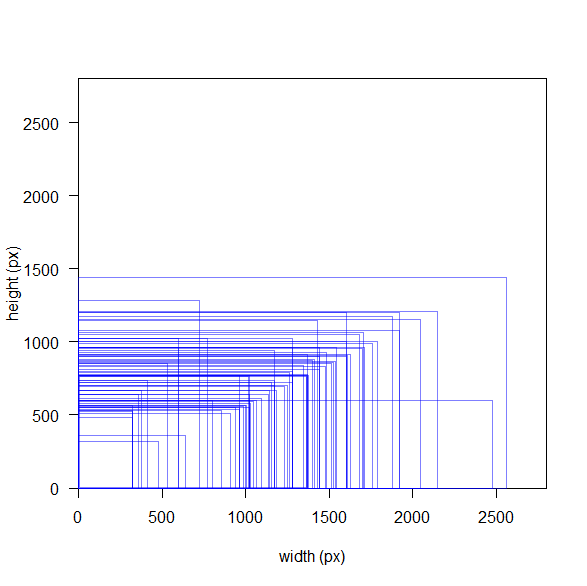
\includegraphics[height=\textheight]{images/devicesizes.png}
\end{center}
}

\frame{

\frametitle{Aside: Unique features of online studies}

\begin{itemize}
\item<2-> Capacity for audio-visual treatments and measurements
\item<3-> Paradata collection
	\begin{itemize}
	\item Implicit outcomes like response times, answer switching, mouse click behavior, browser focus, eye tracking, etc.
	\end{itemize}
\item<4-> Complex randomization (Thursday)
\item<5-> Panel data (Friday)
\item<5-> Synchronous, multi-person designs
\end{itemize}

}



\frame{
\frametitle{``Task'' Designs}

\begin{itemize}\itemsep0.5em
\item Task designs ask respondents to perform a task
\item Often developed for laboratory settings
\item<2-> Most common example: writing something
\item<3-> Can be problematic:
	\begin{itemize}
	\item Time-intensive
	\item Invites drop-off
	\item Compliance problems
	\end{itemize}
\end{itemize}

}


\againframe{ambivalentpartisan}





\questions


\frame{

\frametitle{Sensitive Item Designs}

\begin{itemize}
\item Experiments can also be used to measure something
\item Goal here is not necessarily causal inference, though the causal insight of the experiment provides \textit{descriptively} useful information
\item Paradigms
	\begin{itemize}
	\item List experiments
	\item Endorsement experiments
	\end{itemize}
\end{itemize}
}

\frame{

\frametitle{{\normalsize List Experiments \footnote{Kuklinski et al. 1997. ``Racial Prejudice and Attitudes Toward Affirmative Action.'' \textit{American Journal of Political Science} 41(2): 402--419.}}}

\small

Now I'm going to read you three things that sometimes make people angry or upset. After I read all three, just tell me \textit{how many} of them upset you. I don't want to know which ones. just \textit{how many}.

\footnotesize

\begin{enumerate}
\item the federal government increasing the tax on gasoline
\item professional athletes getting million-dollar salaries
\item large corporations polluting the environment
\item<2-> \textbf{a black family moving in next door}
\end{enumerate}


}

\frame{

\frametitle{{\normalsize Endorsement experiments\footnote{Lyall, Blair, \& Imai. 2013. ``Explaining Support for Combatants during Wartime: A Survey Experiment in Afghanistan.'' \textit{American Political Science Review} 107(4): 679--705.}}}

\small

A recent proposal \only<2>{\textbf{by the Taliban}} calls for the sweeping reform of the Afghan prison system, including the construction of new prisons in every district to help alleviate overcrowding in existing facilities. Though expensive, new programs for inmates would also be offered, and new judges and prosecutors would be trained. How do you feel about this proposal?
}








\section{Surveys in Larger Designs}
\frame{\tableofcontents[currentsection]}

% quasi-experiments and field experiments


\frame{

\frametitle{{\normalsize Field Designs}}

\begin{itemize}\itemsep0.5em
\item Surveys can be used as a measurement instrument for a field treatment
\item No manipulation in the survey itself
\item Survey only measures outcomes
\item<2-> Common uses:
	\begin{itemize}
	\item Post test only Design
	\item Pre-post Design
	\end{itemize}
\item<3-> Problems? Compliance \& nonresponse
\end{itemize}

}



\frame{

\frametitle{{\normalsize Randomized Treatment}}

\small

\begin{itemize}\itemsep-0.2em
\item Examples:
	\begin{enumerate}
	\item<2-> Citizens randomly sent a letter by post encouraging them to reduce water usage
	\item<3-> Different local media markets randomly assigned to receive different advertising
	\end{enumerate}
\item<4-> Survey is used to measure outcomes, when treatment assignment is already known
\end{itemize}

}




\frame{

\frametitle{{\normalsize Quasi-Experimental Treatment}}

\small

\begin{itemize}\itemsep-0.2em
\item Quasi-Experiments are situations where randomization-like forces influence the values of independent variables
	\begin{itemize}
	\item Often ``natural'' experiments where boundaries, discontinuities, or interruptions disrupt treatment-assignment
	\end{itemize}
\item<2-> Examples:
	\begin{itemize}
	\item<2-> Respondents are randomly assigned to be interviewed before or after an event
	\item<3-> Respondents interviewed before \textit{and} after an event that ``randomly'' affects only some, with within-subjects comparisons
	\end{itemize}
\end{itemize}

}

\frame{

\frametitle{Albertson and Lawrence}

What's this study about? What is their quasi-experimental design?

}


\frame{

\frametitle{Within-Subjects Designs}



}


\frame{
	\frametitle{Difference-In-Differences}
	\small
	\begin{itemize}\itemsep0.5em
		\item How do we know change in $Y$ wasn't due to something else?
			\begin{itemize}
				\item How do we know $Y_{0,t}$ is a good stand-in for $Y_{0,t+1}$?
			\end{itemize}
		\item<2-> Use a comparison case (or cases)!
		\item<3-> Instead of using the pre-post difference in $Y_i$ to estimate the causal effect, use the difference in pre-post differences for two units $i$ and $j$:
		\begin{align*}
		(Y_{i,t+1} - Y_{i,t}) - (Y_{j,t+1} - Y_{j,t})
		\end{align*}
	\end{itemize}
}



\frame{

	\frametitle{{\normalsize Threats to Validity}}
	
	\small
	
	As soon as treatment is not truly random, we have to worry about threats to validity.\footnote{Shadish, Cook, and Campbell (2002)}
	
	\begin{enumerate}
	\item<2-> History (simultaneous cause)
	\item<3-> Maturation (time trends)
	\item<4-> Testing (observation changes respondents)
	\item<5-> Instrumentation (changing operationalization)
	\item<6-> Instability (measurement error)
	\item<7-> Attrition
	\end{enumerate}
}


\frame{
	\begin{center}
	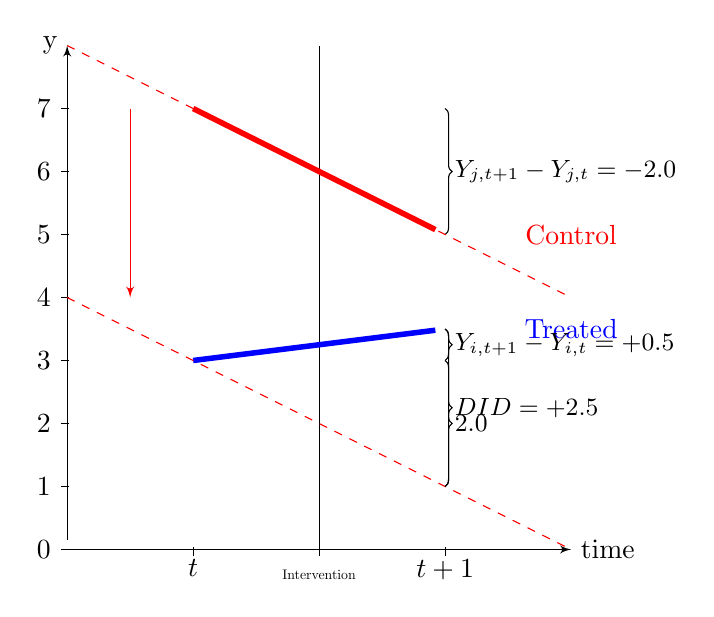
\begin{tikzpicture}[>=latex', scale=0.8]
        \draw[->] (0,0) node (origin) {}  -- (8,0) node[right] (xaxis) {time};
        \draw[->] (origin) -- (0,8) node[left] (yaxis) {y};
        % x ticks
        \foreach \x in {2,4,6}
        	\draw (\x,1pt) -- (\x,-3pt) node[anchor=north] {};
        \draw (2,0) node[below] (before) {$t$};
        \draw (6,0) node[below] (after) {$t+1$};
        \draw (4,-0.25) node[below, scale=0.5] (IV) {Intervention};
        % y ticks
        \foreach \y in {0,...,7}
             \draw (1pt,\y) -- (-3pt,\y) node[anchor=east] {$\y$};
        % intervention
        \draw (4,0) -- (4,8);

        % line
        \draw<2-> (6,3.5) node (tr) {};
        \draw<3-> (6,5) node (ctrl) {};
        \draw<2-3>[blue] (8,3.5) node (trlab) {Treated};
        \draw<3-3>[red] (8,5) node (ctrllab) {Control};        
        \draw<2->[blue, line width=2pt] (2,3) -- (tr);
        \draw<3->[red, line width=2pt] (2,7) -- (ctrl);
        
        % diffs
        \draw<4-6>[right,decorate,decoration={brace,mirror}] 
        	(6,3) -- (6,3.5) node[right, pos=0.5] (idiff) {\small $Y_{i,t+1} - Y_{i,t} = +0.5$};
        \draw<4-6>[right,decorate,decoration={brace}] 
            (6,7) -- (6,5) node[right, pos=0.5] (jdiff) {\small $Y_{j,t+1} - Y_{j,t} = -2.0$};
        
        % trends
        \draw<5-6>[red,->] (1,7) -- (1,4);
        \draw<5->[red, dashed] (0,8) -- (8,4);
        \draw<5->[red, dashed] (0,4) -- (8,0);
        \draw<6>[right,decorate,decoration={brace}] 
            (6,3) -- (6,1) node[right, pos=0.5] (idiff2) {\small $2.0$};
        \draw<7>[right,decorate,decoration={brace}] 
            (6,3.5) -- (6,1) node[right, pos=0.5] (idiff2) {\small $DID = +2.5$};
                        
        
    \end{tikzpicture}
    \end{center}
}




\frame{
	\frametitle{{\large Local Average Treatment Effect}}
	\small
	\begin{itemize}\itemsep0.2em
	\item IV estimate \textit{local} to the variation in $X$ that is due to variation $W$ (i.e., the LATE)
	\item This matters if effects are \textit{heterogeneous}
	\item LATE is effect for those who \textit{comply} with instrument
	\item Four subpopulations:
		\begin{itemize}\footnotesize
		\item Compliers: $X = 1$ only if $W = 1$
		\item Always-takers: $X = 1$ regardless of $W$
		\item Never-takers: $X = 0$ regardless of $W$
		\item Defiers: $X = 1$ only if $W = 0$
		\end{itemize}
	\end{itemize}
}

\frame{
	\frametitle{How IV Works II (Wald)}
	\small
	\begin{itemize}\itemsep0.5em
		\item Imagine two effects:
		\begin{align}
		ITT_y & = E[y_i | w_i = 1] - E[y_i | w_i = 0]\\
		ITT_x & = E[x_i | w_i = 1] - E[x_i | w_i = 0]
		\end{align}
		\item IV estimates the LATE: $\dfrac{ITT_y}{ITT_x}$
		\item In a regression, this is:\\
			$E[y_i|w_i] = \beta_0 + \text{LATE} \times E[x_i|w_i]$
	\end{itemize}
}



\frame{
	\frametitle{What is ``instrumental''?}
	\begin{itemize}\itemsep1em
		\item $W$ must be a crucial cause of $X$'s effect on $Y$
		\item $W$ is the quasi-experimental shock to the causal process in our graph
			\begin{itemize}
			\item It is not caused by $X$ or $Y$
			\item It does not cause $Y$ except through $X$
			\end{itemize}
	\end{itemize}	
}





\questions

\frame{

\frametitle{Homework!}

\begin{itemize}
\item Working alone, with a partner, or in a small group, start thinking about a possible experiment
\item Start writing a protocol:
	\begin{enumerate}
	\item Theory/hypotheses
	\item Instrumentation
	\end{enumerate}
\item Time on Friday to share and get feedback
\end{itemize}

}



\appendix
\frame{}

\end{document}
